\section{Entscheidbarkeit}

\subsection{Entscheidbarkeit}
Eine Sprache $A \subset \Sigma^*$ heisst \textbf{entscheidbar}, wenn eine TM $T$ existiert, die das Entscheidungsproblem $(\Sigma, A)$ löst:
\begin{itemize}
    \item $x \in A \Rightarrow T$ hält mit Bandinhalt ``1'' (Ja)
    \item $x \in \Sigma^* \setminus A \Rightarrow T$ hält mit Bandinhalt ``0'' (Nein)
\end{itemize}
$T$ muss bei \textbf{jeder} Eingabe $x \in \Sigma^*$ nach endlich vielen Schritten halten.\\
Äquivalent: $A$ ist entscheidbar $\Leftrightarrow$ $(\Sigma, A)$ mit einem WHILE-Programm lösbar (Entscheidungsverfahren).

\subsection{Semi-Entscheidbarkeit}
$A \subset \Sigma^*$ heisst \textbf{semi-entscheidbar}, wenn eine TM $T$ existiert mit:
\begin{itemize}
    \item $x \in A \Rightarrow T$ hält mit Bandinhalt ``1'' (Ja)
    \item $x \in \Sigma^* \setminus A \Rightarrow T$ hält \textbf{nie} an
\end{itemize}
Liefert nur positive Antworten; statt ``Nein'' keine Antwort.

\subsection{Konvention (natürliche Zahlen)}
$X \subset \mathbb{N}$ ist (semi-) entscheidbar $\Leftrightarrow$ $\{bin(x) \mid x \in X\} \subset \{0,1\}^*$ ist (semi-) entscheidbar.

\subsection{Zusammenhänge}
\begin{itemize}
    \item Jede entscheidbare Sprache ist auch semi-entscheidbar.
    \item $A$ ist entscheidbar $\Leftrightarrow$ sowohl $A$ als auch $\overline{A}$ sind semi-entscheidbar.
\end{itemize}
\textbf{Beweis ($\Leftarrow$):} Simuliere semi-Entscheidungsverfahren für $A$ und $\overline{A}$ schrittweise parallel:
\begin{verbatim}
INPUT(w); n = 0;
WHILE true DO
  n = n + 1;
  IF A(w,n) THEN return 1;
  IF B(w,n) THEN return 0
END
\end{verbatim}
$A(w,n)$: semi-EV von $A$ terminiert nach $n$ Schritten;\\$B(w,n)$: analog für $\overline{A}$.

\subsection{Abschlusseigenschaften}
\begin{itemize}
    \item $A$ entscheidbar $\Rightarrow$ $\overline{A}$ entscheidbar
    \item $A, B$ (semi-) entscheidbar $\Rightarrow$ $A \cup B$, $A \cap B$ (semi-) entscheidbar
\end{itemize}

\subsection{Charakterisierungen (Semi-Entscheidbarkeit)}
Für $A \subset \Sigma^*$ sind äquivalent:
\begin{itemize}
    \item $A$ ist rekursiv aufzählbar
    \item $A$ ist semi-entscheidbar
    \item $A$ ist Wertebereich einer totalen berechenbaren Funktion
    \item $A$ ist Definitionsbereich einer berechenbaren Funktion
\end{itemize}

\subsection{Reduktion}
$A \subset \Sigma^*$ heisst auf $B \subset \Gamma^*$ \textbf{reduzierbar} ($A \preceq B$), wenn es eine totale, Turing-berechenbare Funktion $F : \Sigma^* \to \Gamma^*$ gibt mit:
\[
    w \in A \Longleftrightarrow F(w) \in B
\]

\textbf{Transitivität:} $A \preceq B$ und $B \preceq C \Rightarrow A \preceq C$\\
\textbf{Satz:} Ist $B$ (semi-) entscheidbar und $A \preceq B$, dann ist auch $A$ (semi-) entscheidbar.\\
\textbf{Kontraposition:} Ist $A$ unentscheidbar und $A \preceq B$, dann ist auch $B$ unentscheidbar.\\
\textbf{Beweis (Entscheidbarkeit):}
\begin{verbatim}
INPUT(w); u = F(w); RETURN P(u)
\end{verbatim}

\subsection{Halteprobleme}

\subsubsection{Spezielles Halteproblem}
$H_S := \{w \in \{0,1\}^* \mid T_w \text{ angesetzt auf } w \text{ hält}\}$\\
\textbf{Gegeben:} Code $w$ einer TM $T_w$. \\
\textbf{Gefragt:} Hält $T_w$ auf eigenem Code $w$?

\subsubsection{Allgemeines Halteproblem}
$H := \{w\#x \in \{0,1,\#\}^* \mid T_w \text{ angesetzt auf } x \text{ hält}\}$\\
\textbf{Gegeben:} Code $w$ einer TM $T_w$ und Input $x$. \\
\textbf{Gefragt:} Hält $T_w$ auf Eingabewort $x$?

\subsubsection{Leeres Halteproblem}
$H_0 := \{w \in \{0,1\}^* \mid T_w \text{ angesetzt auf $\varepsilon$ Band hält}\}$\\
\textbf{Gegeben:} Code $w$ einer TM $T_w$. \\
\textbf{Gefragt:} Hält $T_w$ auf leerem Band?

\subsection{Unentscheidbarkeit der Halteprobleme}

\subsubsection{Unentscheidbarkeit von $H_S$}
Annahme: TM $T$ entscheidet $H_S$. Konstruiere TM $P$:
\begin{center}
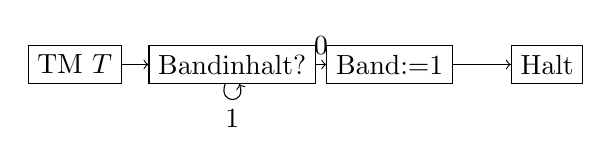
\begin{tikzpicture}[node distance=2cm, auto]
  \node (T) [draw, rectangle] {TM $T$};
  \node (check) [draw, rectangle, right of=T] {Bandinhalt?};
  \node (set) [draw, rectangle, right of=check] {Band:=1};
  \node (halt) [draw, rectangle, right of=set] {Halt};
  
  \draw [->] (T) -- (check);
  \draw [->] (check) -- node[above] {0} (set);
  \draw [->] (set) -- (halt);
  \draw [->] (check) to [out=250,in=290,looseness=4] node[below] {1} (check);
\end{tikzpicture}
\end{center}
Sei $w$ der Code von $P$ ($T_w = P$):
\begin{itemize}
    \item $P$ auf $w$ hält $\Leftrightarrow T(w)=0 \Leftrightarrow T_w$ auf $w$ hält nicht $\Leftrightarrow P$ auf $w$ hält nicht $\lightning$
\end{itemize}

\subsubsection{Unentscheidbarkeit von $H$}
Reduktion $H_S \preceq H$ via $F(x) = x\#x$.\\
$w \in H_S \Leftrightarrow T_w$ hält auf $w \Leftrightarrow w\#w \in H \Leftrightarrow F(w) \in H$

\subsubsection{Unentscheidbarkeit von $H_0$}
Reduktion $H \preceq H_0$: Für Input $w\#x$ konstruiere TM $T'$, die zuerst $x$ auf das leere Band schreibt und sich dann wie $T_w$ verhält.\\
$T_w$ hält auf $x \Leftrightarrow T'$ hält auf leerem Band.

\subsection{Semi-Entscheidbarkeit der Halteprobleme}
$H_0$, $H_S$ und $H$ sind semi-entscheidbar.\\
Wegen $H_S \preceq H \preceq H_0$ genügt es, $H_0$ als semi-entscheidbar nachzuweisen: Universelle TM $U$ simuliert $T_w$ auf leerem Band; falls $U$ hält $\to$ Band $:= 1$.

\subsection{Satz von Rice}
Ist $R$ die Menge aller berechenbaren Funktionen und $S \subset R$ eine \textbf{echte, nichtleere} Teilmenge, dann ist
\[
    C(S) = \{w \in \{0,1\}^* \mid F_w \in S\}
\]
\textbf{unentscheidbar}.\\
\textbf{Konsequenzen:} Es ist im Allgemeinen unmöglich mechanisch zu prüfen, ob ein Programm\ldots
\begin{itemize}
    \item eine bestimmte Spezifikation erfüllt
    \item frei von Bugs ist
    \item bei jeder Eingabe terminiert
    \item dieselbe Funktionalität wie ein anderes Programm hat
\end{itemize}